% !TeX root = ../apuntes-ea.tex

\chapter{Homomorfismos de anillos}

\section{Extensión desde los homomorfismos de grupos.}

Solo necesitamos definir qué tiene que pasar con la segunda operación. Si lo hacemos bien, todas las propiedades se mantienen.

\begin{dfn}[Homomorfismo de anillos]
	Sean $(A, +, \cdot), (B, \oplus, \odot)$ anillos y sea $\varphi: A \to B$. Decimos que $\varphi$ es un homomorfismo de anillos si
	\begin{enumerate}
		\item $\varphi(a_1+a_2) = \varphi(a_1) \oplus \varphi(a_2)$
		\item $\varphi(a_1 \cdot a_2) = \varphi(a_1)\odot\varphi(a_2)$
		\item $\varphi(\1_A) = \1_B$
	\end{enumerate}
\end{dfn}

\begin{obs}
	Dado $\varphi:A \to B$ homomorfismo de anillos, $\ima \varphi \subset B$ siempre es un subanillo de $B$.
\end{obs}

\begin{pro}[Inyectividad/sobreyectividad en homomorfismos de anillos]
	Sea $\varphi: A \to B$ un homomorfismo de anillos.
	\begin{itemize}
		\item $\varphi$ inyectivo $\iff \ker \varphi = \{\0\}$
		\item $\varphi$ sobre $\iff \ima \varphi = B$
	\end{itemize}
\end{pro}

\begin{pro}
	El homomorfismo de anillos $\varphi: A \to B$ es una biyección de conjuntos $\iff \ker \varphi = \{\0\} \land \ima \varphi = B$.
\end{pro}

\begin{obs}
	Si $\varphi:A \to B$ homomorfismo de anillos es una biyección de conjuntos entonces $\inv{\varphi}:B \to A$ también es un homomorfismo de anilos.
\end{obs}

\begin{dfn}[Isomorfismo de anillos]
	Diremos que un homomorfismo de anillos $\varphi:A \to B$ es un isomorfismo de anillos $\iff \exists \inv{\varphi} : B \to A$ tal que
	\begin{align*}
	\varphi \circ \inv{\varphi} = Id_B \land \inv{\varphi} \circ \varphi = Id_A
	\end{align*}
\end{dfn}

\begin{pro}
	Sea $\varphi:A \to B$ un homomorfismo de anillos. Entonces $\varphi$ es un isomorfismo de anillos $\iff \ker \varphi = \{\0\} \land \ima \varphi = B$.
\end{pro}

\section{Homomorfismos de anillos y divisores de $\0$}

\begin{ej}
	Sea $s \in A,\ s\neq \0$. Fijado $s$, definimos $\alpha_s : A \to A, a \mapsto a\cdot s$. Observemos:
	\begin{enumerate}
		\item $\alpha_s$ es un homomorfismo de grupos
		\item $\alpha_s$ es inyectivo $\iff \ker \alpha_s = \{ \0 \}$
		\begin{itemize}
			\item $\ker \alpha_s = \{\0\} \iff s$ no es divisor de $\0$
			\item $\ker \alpha_s \neq \{\0\} \iff s$ es divisor de $\0$
		\end{itemize}
		\item $\ima \alpha_s = \gen{\{s\}}$
		\begin{itemize}
			\item $s \in \uds{A} \iff \gen{s}$ (ver \autoref{pro:inunidadesiffgenerado}), por tanto $\alpha_s$ es sobre $\iff \ima \alpha_s = A \iff \gen{s} = A \iff s \in \uds{A}$.
		\end{itemize}
		
	\end{enumerate}
\end{ej}

Este ejemplo nos permite dar el siguiente teorema:

\begin{thm}
	Sea $(A, +, \cdot)$ un anillo finito y sea $a \in A \setminus \{\0\}$. Entonces, o bien $a \in \uds{A}$, o bien $a$ es un divisor de $\0$. Por tanto escribimos
	\begin{align*}
	A \setminus \{\0\} = \uds{A} \bigcup_{\text{disjunta}} \{a \in A \mid a \text{ divisor de }\0\}
	\end{align*}
\end{thm}

\begin{proof}
	Fijo $s \in A \setminus \{\0\}$. Como $A$ es finito $\alpha_s$ inyectiva $\iff \alpha_s$ sobreyectiva $\iff \alpha_s$ biyectiva. Entonces, fijándonos en el ejemplo anterior, tenemos
	\begin{itemize}
		\item Si $s \in \uds{A}$ entonces $\alpha_s$ inyectiva\footnote{Esto es porque $\forall a,b \in A, \alpha_s(a) = \alpha_s(b) \iff sa = sb \iff \inv{s}sa = \inv{s}sb \iff a = b \implies \alpha_s$ inyectiva. Ver ejercicio \autoref{ex:h5.4} para más detalles en la demostración de este teorema.} $\implies \ker \alpha_s = \{\0\} \implies s$ no es un divisor de $0$.
		\item Si $s \notin \uds{A}$ entonces $\alpha_s$ no es sobre $\implies \alpha_s$ no inyectiva $\implies \ker \alpha_s \neq \{\0\} \implies s$ es un divisor de $\0$.
	\end{itemize}
\end{proof}

\begin{ej}
	Sea $A = \Z/8\Z \times \Z/10\Z$. ¿Cuántos divisores de $\0$ tiene $A$?
\end{ej}

\begin{proof}
	Sabemos que $|A| = 80 \implies A \setminus \{\0\}$ tiene 79 elementos. Además, por la \autoref{pro:udsproductodirectoanillos}, sabemos que $\uds{A} = \uds{\Z/8\Z} \times \uds{\Z/10\Z} \implies |\uds{A}| = 4 \times 4 = 16$. Luego hay $79 - 16 = 63$ divisores de $\0$ en $A$.
\end{proof}

\section{Homomorfismos de anillos e ideales}

\subsection{Relación de equivalencia inducida por los ideales}

\begin{dfn}[Relación de equivalencia por ideales]
	Sea $I \subset A$ un ideal. Definimos la relación de equivalencia $a_1 R a_2 \iff a_1 - a_2 \in I$.
\end{dfn}

\begin{pro}
	$R$ es efectivamente una relación de equivalencia
\end{pro}

\begin{proof}Probamos las 3 propiedades de las relaciones de equivalencia:
	\begin{enumerate}
		\item Reflexiva: $\forall a_1 \in A,\ a_1 - a_1 = \0 \in I \implies a_1Ra_1$
		\item Simétrica: $\forall a_1, a_2 \in A$ con $a_1 R a_2$ tenemos que $a_2 - a_1 = -(a_1 - a_2) \in I \implies a_2 R a_1$
		\item Transitiva: $a_1Ra_2 \land a_2Ra_3 \implies (a_1 - a_2) \in I \land (a_2 - a_3) \in I \implies ((a_1 - a_2) - (a_2 - a_3) \in I \implies (a_1 - a_3) \in I \implies a_1 R a_3$
	\end{enumerate}
\end{proof}

¿Cómo son las clases de equivalencia que viven en el conjunto cociente $A/I$? Pues son de la forma $\overline{a} = a + I = \{a + i_i \mid i_i \in I\}$. Podemos dotar de estructura de anillo a este conjunto cociente. Las operaciones que definimos son las naturales:

\begin{dfn}[Estructura de anillo del cociente]
	Sea $(A, +, \cdot)$ un anillo, $I \subset A$ un ideal. La relación de equivalencia $a_1 R a_2 \iff a_1 - a_2 \in I$ define una partición en clases de equivalencia $\overline{a} \in A/I$. Definimos las operaciones $\#$ y $\bullet$
	
	\begin{align}
	\overline{a} \# \overline{b} = a + i_i + b + i_j = a+b + \underbrace{i_i + i_j}_{\in I} = \overline{a+b} \\
	\overline{a}\bullet\overline{b} = (a+i_i)(b+i_i) = ab + \underbrace{a i_i + b i_j + i_i i_j}_{\in I} = \overline{a \cdot b}
	\end{align}
	De este modo $(A/I, \#, \bullet)$ es un anillo y $\pi: A \to A/I$ definido con $a \mapsto \pi(a) = \overline{a}$ es un homomorfismo de anillos.
\end{dfn}

Hemos esperado a dar esto hasta ahora para poder dar la definición correcta del homomorfismo de anillos $\pi$ que aparece al crear el cociente.

\begin{pro}
	Lo que dice la definición es verdad: $(A/I, \#, \bullet)$ es un anillo y $\pi$ un homomorfismo de anillos.
\end{pro}

\begin{pro}
	La función $\pi: A \to A/I$ que da las clases de equivalencia es un epimorfismo de grupos (es sobreyectivo) y además $\ker \pi = I$.
\end{pro}

\begin{pro}
	$P \subset A$ ideal primo $\iff A/P$ es un dominio de integridad
\end{pro}

\begin{figure}[h]
	\centering
	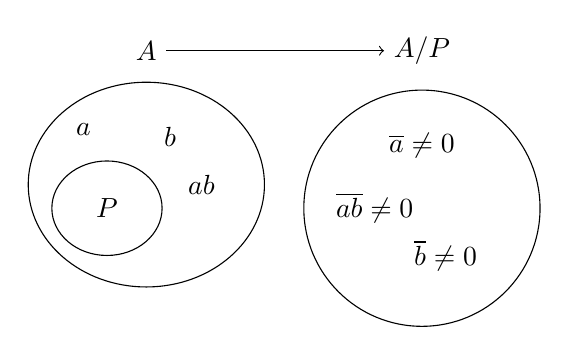
\begin{tikzpicture}
	% TODO: poner puntitos en los nodos
	\node (a) at (-0.3,1) {$a$};
	\node (b) at (0.8,0.9) {$b$};
	\node (ab) at (1.2, .3) {$ab$};
	\node (P) at (0,0) {$P$};
	\node (A) at (0.5,2) {$A$};
	
	\draw (P) ellipse (.7 and .6);
	\draw (0.5,0.3) ellipse (1.5 and 1.3);
	
	\begin{scope}[shift={(4,0)}]
	\node (AP) at (0, 2) {$A/P$};
	\node (abp) at (-.6, 0) {$\overline{ab} \neq 0$};
	\node (ap) at (0, .8) {$\overline{a} \neq 0$};
	\node (bp) at (0.3,-.6) {$\overline{b} \neq 0$};
	\draw (0,0) ellipse (1.5 and 1.5);
	\end{scope}
	\draw[->] (A) -- (AP);
	\end{tikzpicture}
\end{figure}

\begin{proof}
	Sabemos que
	\begin{align*}
	a \notin P &\iff \overline{a} \neq \overline{\0} \text{ en } A/P \\
	b \notin P &\iff \overline{b} \neq \overline{\0} \text{ en } A/P \\
	a\cdot b \notin P &\iff \overline{a\cdot b} = \overline{a}\cdot \overline{b} \neq \overline{\0} \text{ en } A/P
	\end{align*}
	Luego es claro que $P$ ideal primo $\iff$ el producto de elementos no nulos es no nulo en $A/P \iff A/P$ es un DI (dominio de integridad).
\end{proof}


\subsection{Retículo de ideales}

% TODO
\begin{dfn}[Retículo de ideales]
	Estaría bien tener una definición de esto.
\end{dfn}


\begin{ej}
	En $(\Z/8\Z, +, \cdot)$ el retículo de ideales coincide con los subgrupos de $(\Z/8\Z, +)$:
	\begin{align*}
	\{\overline{0}\} \subset \gen{\overline{4}} = \{\overline{0}, \overline{4}\} \subset \gen{\overline{2}} = \{\overline{0}, \overline{2}, \overline{4}, \overline{6}\} \subset \Z/8\Z
	\end{align*}
\end{ej}

\subsection{Correspondencia entre ideales por un epimorfismo de anillos}

Ahora damos un teorema análogo al de correspondencia que dimos para subgrupos (\autoref{thm:correspondenciasubgrupos}).

\begin{thm}[de correspondencia entre ideales]
	Sean $A$ y $B$ anillos y sea $\alpha: A \to B$ un homomorfismo de anillos.
	\begin{enumerate}
		\item Si $J \subset B$ es un ideal entonces $\alpha^{-1}(J)$ es un ideal en $A$.
		\item Si $I \subset A$ es un ideal y además $\alpha$ es sobreyectivo entonces la imagen $\alpha(I)$ es un ideal en $B$.
	\end{enumerate}
\end{thm}

\begin{proof}[Demostración de 1]
	\begin{figure}[h]
		\centering
		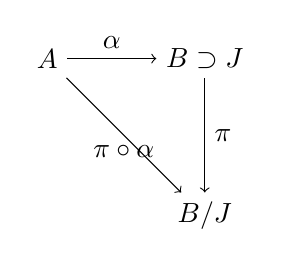
\begin{tikzpicture}
		\node (A) at (0,0) {$A$};
		\node (B) at (2,0) {$B \supset J$};
		\node (BJ) at (2,-2) {$B/J$};
		
		\draw[->] (A) -- (B) node[pos=.5, above] {$\alpha$};
		\draw[->] (B) -- (BJ) node[pos=.5,right] {$\pi$};
		\draw[->] (A) -- (BJ) node[pos=.5,below] {$\pi \circ \alpha$};
		\end{tikzpicture}
	\end{figure}
	Observar que $\alpha^{-1}(J) = \ker (\pi \circ \alpha)$ y por tanto es un ideal.
\end{proof}

\begin{proof}[Demostración de 2]
	Probamos las 3 propiedades de los ideales (definición de Orlando, \autoref{dfn:idealorlando}).
	\begin{enumerate}
		\item $\0 \in I \land \alpha$ h. de anillos $\implies \alpha(\0) = \0 \in \alpha(I)$
		\item Sean $\alpha(b_1), \alpha(b_2) \in \alpha(I)$. Entonces $\exists a_1, a_2 \in I \mid b_1 = \alpha(a_1) \land b_2 = \alpha(a_2)$. Por tanto $b_1 + b_2 = \alpha(a_1 + a_2) = \alpha(a_1) + \alpha(a_2) \in I \implies b_1 + b_2 \in \alpha(I)$.
		\item Sea $b \in B$. Como $\alpha$ es sobre, $\exists a \in A \mid \alpha(a) \in B$. Sea $b' \in \alpha(I) \implies \exists a' \in I \mid b' = \alpha(a')$. Entonces $bb' = \alpha(a) \alpha(a') = \alpha(aa') \in \alpha(I)$ porque $aa' \in I$.
	\end{enumerate}
\end{proof}

\begin{pro}
	\label{pro:correspondenciaideales2}
	Sea $(A, +, \cdot)$ un anillo, $I \subsetneq A$ un ideal propio de $A$. Sea $\pi: A \to A/I$ la función sobreyectiva que da las clases de equivalencia para cada elemento $a \in A \mapsto \overline{a}$ que tiene $\ker \pi = I$. Se tiene
	\begin{enumerate}
		\item Si $\overline{J}$ es un ideal en $A/I$ entonces $\inv{\pi}(\overline{J})$ es un ideal en $A$ que contiene a $I$
		\item Si $J$ es un ideal en $A$ entonces $\pi(J)$ es un ideal en $A/I$ y $J \subset \inv{\pi}(\pi(J))$.
		\begin{itemize}
			\item Si además $I \subset J$ entonces hay igualdad $J = \inv{\pi}(\pi(J))$.
		\end{itemize}
	\end{enumerate}
\end{pro}

\begin{proof}
	Si $\overline{J}$ es un ideal en $A/I$.
	
	\begin{figure}[h]
		\centering
		\begin{tikzpicture}
		\node (A) at (0,0) {$A$};
		\node (AI) at (2,0) {$A/I \supset \overline{J}$};
		\node (AIJ) at (2,-2) {$\frac{A/I}{\overline{J}}$};
		
		\draw[->] (A) -- (AI) node[pos=.5, above] {$\pi$};
		\draw[->] (AI) -- (AIJ) node[pos=.5,right] {$\pi'$};
		\end{tikzpicture}
	\end{figure}
	La composición $\pi' \circ \pi$ es un homomorfismo de anillos y además $\ker (\pi' \circ \pi) = \inv{\pi}(\overline{J})$
\end{proof}

\begin{obs}
	El ideal $\{\overline{\0}\}$ de $A/I$ tiene contraimagen $\inv{\pi}(\{\overline{\0}\}) = I$.
\end{obs}

\begin{ej}
	Buscamos el retículo de ideales del grupo $\Z/8\Z$. Por la \autoref{pro:correspondenciaideales2} tenemos que los ideales $\overline{J}$ de $\Z/8\Z$ están en correspondencia con los ideales $J$ en a que contengan a $8\Z$ (Aquí $A = \Z,\ I = 8\Z$).
	
	\begin{figure}[h]
		\centering
		\begin{tikzpicture}
			% end nZ
			\node (z) at (-3,2) {$\Z = \gen{1}$};
			\node (2z) at (-3,1) {$2\Z = \gen{2}$};
			\node (4z) at (-3,0) {$4\Z = \gen{4}$};
			\node (8z) at (-3,-1) {$8\Z = \gen{8}$};
			
			\draw (8z) -- (4z);
			\draw (4z) -- (2z);
			\draw (2z) -- (z);
			
			% en Z/nZ
			\node (z8) at (0,2) {$\gen{\overline{1}} = \Z/8\Z$};
			\node (z4) at (0,1) {$\gen{\overline{2}} = \{\overline{\0}, \overline{2}, \overline{4}, \overline{4}\}$};
			\node (z2) at (0,0) {$\gen{\overline{4}} = \{\overline{\0}, \overline{4}\}$};
			\node (e) at (0,-1) {$\gen{\overline{8}} = \{\overline{\0}\}$};
			
			\draw (e) -- (z2);
			\draw (z2) -- (z4);
			\draw (z4) -- (z8);
			
			% las correspondencias
			\draw (z)  edge[->, blue] (z8);
			\draw (2z) edge[->, blue] (z4);
			\draw (4z) edge[->, blue] (z2);
			\draw (8z) edge[->, blue] (e);
		\end{tikzpicture}
		\caption{Retículo de ideales del anillo $\Z/12\Z$ en correspondencia con los ideales de $\Z$ que contienen a $12\Z$.}
	\end{figure}

	Obtenemos cada ideal de $\Z/12\Z$ aplicando $\pi$ a cada ideal de $\Z$ que contiene a $12\Z$, esto es, cogiendo cada uno de sus elementos y tomando su clase. Para simplificar el dibujo, hemos puesto los ideales con generadores pero se puede hacer a mano. También se puede hacer directamente tomando la imagen del generador de un ideal de $\Z$ que contiene a $12\Z$.
\end{ej}


\begin{ej}
	Buscamos el retículo de ideales de $\Z/12\Z$. Aplicanto la \autoref{pro:correspondenciaideales2} tomando $A = \Z, I = 12\Z$, sabemos que los ideales del retículo de $\Z/12\Z$ están en correspondencia con los del retículo de $\Z$ que contienen al $12\Z$.
	
	\begin{figure}[h]
		\centering
		\begin{tikzpicture}
			\node (z) at (0,0) {$\Z$};
			\node (2z) at (-1, -1) {$2\Z$};
			\node (3z) at (1,-1) {$3\Z$};
			\node (4z) at (-2, -2) {$4\Z$};
			\node (6z) at (0,-2) {$6\Z$};
			\node (12z) at (-1, -3) {$12\Z$};
			
			\draw (12z) -- (4z) -- (2z) -- (z);
			\draw (12z) -- (6z) -- (3z) -- (z);
			\draw (6z) -- (2z);
			
			\begin{scope}[shift={(6,-2)}]
			\node (zp) at (0,0) {$\gen{\overline{1}} = \Z/12\Z$};
			\node (2zp) at (-1, -1) {$\gen{\overline{2}}$};
			\node (3zp) at (1,-1) {$\gen{\overline{3}}$};
			\node (4zp) at (-2, -2) {$\gen{\overline{4}}$};
			\node (6zp) at (0,-2) {$\gen{\overline{6}}$};
			\node (12zp) at (-1, -3) {$\gen{\overline{12}} = \{\0\}$};
			
			\draw (12zp) -- (4zp) -- (2zp) -- (zp);
			\draw (12zp) -- (6zp) -- (3zp) -- (zp);
			\draw (6zp) -- (2zp);
			\end{scope}
			
			\draw (z) edge[->, blue, bend left] (zp);
			\draw (2z) edge[->, blue, bend left] (2zp);
			\draw (3z) edge[->, blue, bend right] (3zp);
			\draw (4z) edge[->, blue, bend left] (4zp);
			\draw (6z) edge[->, blue, bend right] (6zp);
			\draw (12z) edge[->, blue, bend right] (12zp);
		\end{tikzpicture}
		\caption{Los ideales de $\Z/12\Z$ en correspondencia con los ideales de $\Z$ que contienen a $12\Z$.}
	\end{figure}
\end{ej}

Como cabría esperar...

\begin{pro}
	En $\Z/n\Z$ hay un ideal por cada divisor positivo de $n$. Además dos ideales $\pi(n\Z)$ y $\pi(m\Z)$ cumplen
	\begin{align*}
		\left(n\Z \subset m\Z \iff m \text{ divide a } n\right) \implies \left(\pi(n\Z) \subset \pi(m\Z) \iff m \text{ divide a } n\right)
	\end{align*}
\end{pro}

\begin{ej}[Retículo de ideales de $(\Z, +, \cdot)$]
	
	Sabemos que los ideales de $\Z$ son de la forma $n\Z = 0\Z, 1\Z, 2\Z, 3\Z, 4\Z, \dots$ para $n = 0,1,2,3,\dots$ Observemos que podemos construir el retículo sabiendo que $n\Z \subset m\Z \iff n \in m\Z\iff m \divides n$. Así nos va quedando el retículo:
	
	\begin{figure}[h]
		\centering
		% TODO sombrear los que contienen al 6
		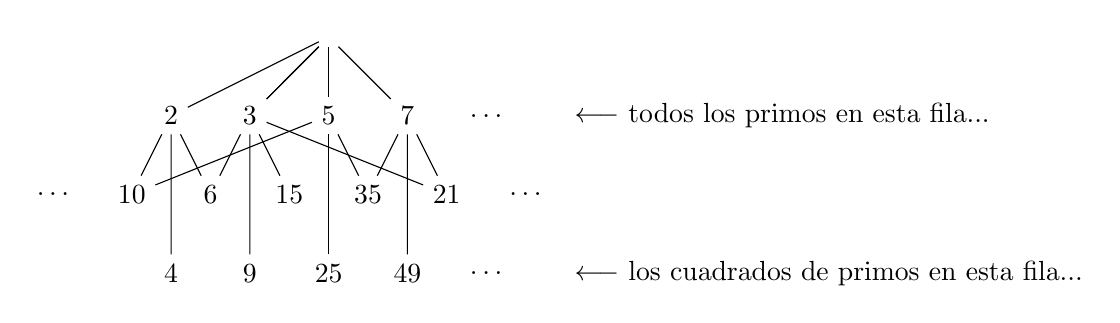
\begin{tikzpicture}
		\node (z) at (0,1) {$\Z$};
		\node (2z) at (-2,0) {$2\Z$};
		\node (3z) at (-1,0) {$3\Z$};
		\node (5z) at (0,0) {$5\Z$};
		\node (7z) at (1,0) {$7\Z$};
		\node (dots) at (2,0) {$\dots$};
		\node[right] (prims) at (3,0) {$\longleftarrow$ todos los primos en esta fila...};
		
		\node (mmdots) at (-3.5,-1) {$\dots$};
		\node (10z) at (-2.5,-1) {$10\Z$};
		\node (6z) at (-1.5,-1) {$6\Z$};
		\node (15z) at (-0.5,-1) {$15\Z$};
		\node (35z) at (0.5,-1) {$35\Z$};
		\node (21z) at (1.5, -1) {$21\Z$};
		\node at (2.5, -1) {$\dots$};
		
		\node (4z) at (-2,-2) {$4\Z$};
		\node (9z) at (-1, -2) {$9\Z$};
		\node (25z) at (0,-2) {$25\Z$};
		\node (49z) at (1, -2) {$49\Z$};
		\node at (2,-2) {$\dots$};
		\node[right] (pprims) at (3,-2) {$\longleftarrow$ los cuadrados de primos en esta fila...};
		
		\draw 	(4z) -- (2z)
		(2z) -- (z);
		\draw 	(9z) -- (3z)
		(3z) -- (z);
		\draw 	(25z) -- (5z)
		(5z) -- (z);
		\draw 	(49z) -- (7z)
		(7z) -- (z);
		\draw	(10z) -- (2z)
		(10z) -- (5z);
		\draw 	(6z) -- (2z)
		(6z) -- (3z);
		\draw	(15z) -- (3z)
		(3z) -- (z);
		\draw	(35z) -- (5z)
		(35z) -- (7z);
		\draw	(21z) -- (3z)
		(21z) -- (7z);
		\end{tikzpicture}
		\caption{Retículo de ideales de $(\Z, +, \cdot)$.}
	\end{figure}
\end{ej}

\begin{obs}
	Ya hemos visto que los ideales maximales de $\Z$ son los de la forma $p\Z$ con $p$ primo. Es natural entonces que $\Z/n\Z$ tenga tantos ideales maximales como divisores primos tenga $n$. Observemos que no importa la multiplicidad ya que los ideales que se corresponden con $p^r,\ r > 1$ no están en la primera fila, sino que están incluidos en ideales que sí están en la primera fila.
\end{obs}

Mira tu por donde...

\begin{pro}
	Sea $(A, +, \cdot)$ un anillo. Son equivalentes:
	\begin{enumerate}
		\item $A$ es un cuerpo.
		\item El retículo de ideales es el trivial, es decir, que solo tiene como ideales a $\{\0\}$ y a sí mismo.
	\end{enumerate}
\end{pro}

\section{Primer teorema de isomorfía para anillos}

\begin{thm}[Primer teorema de la isomorfía para anillos]
	Sea $\alpha: A \to B$ homomorfismo de anillos sobreyectivo. Entonces $B$ es isomorfo a $A/\ker\alpha$.
\end{thm}

El resultado que acabamos de dar a veces se llama Teorema Fundamental de Isomorfismos de Anillos \cite{dor96}. Lo hemos llamado Primer Teorema de la Isomorfía para anillos porque es lo mismo cambiando grupo por anillo y subgrupo normal por ideal.

\begin{figure}[h]
	\centering
	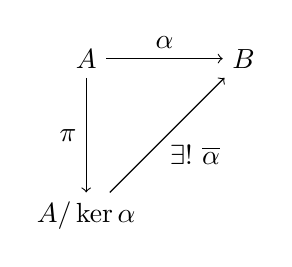
\begin{tikzpicture}
	\node (A) at (0,0) {$A$};
	\node (B) at (2,0) {$B$};
	\node (Aker) at (0, -2) {$A/\ker \alpha$};
	
	\draw[->] (A) -- (B) node[pos=.5, above] {$\alpha$};
	\draw[->] (A) -- (Aker) node[pos=.5,left] {$\pi$};
	\draw[->] (Aker) -- (B) node[pos=.5, below] {$\qquad\exists!\ \overline{\alpha}$};
	\end{tikzpicture}
\end{figure}

Para probarlo nos ayudamos del siguiente Lema:

\begin{lm}
	Sea $\varphi: A \to B$ homomorfismo de anillos. Sea $I$ un ideal en $A$ tal que $I \subset \ker \varphi$.
	\begin{figure}[h]
		\centering
		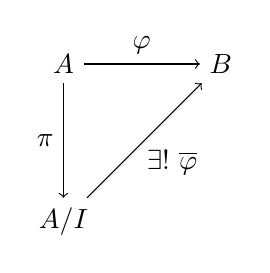
\begin{tikzpicture}
		\node (A) at (0,0) {$A$};
		\node (B) at (2,0) {$B$};
		\node (AI) at (0, -2) {$A/I$};
		
		\draw[->] (A) -- (B) node[pos=.5, above] {$\varphi$};
		\draw[->] (A) -- (AI) node[pos=.5,left] {$\pi$};
		\draw[->] (AI) -- (B) node[pos=.5, below] {$\qquad\exists!\ \overline{\varphi}$};
		\end{tikzpicture}
	\end{figure}
	Entonces:
	\begin{enumerate}
		\item $\exists !\ \overline{\varphi} : A / \ker \varphi \to B$ tal que $\varphi = \overline{\varphi} \circ \pi$
		\item $\ker \overline{\varphi} = \frac{\ker \varphi}{I}$
	\end{enumerate}
\end{lm}

\begin{proof}[Demostración de 1]
	Recordemos que $\pi:A \to A/I$ (la proyección que lleva cada elemento a su clase) es sobre. Tenemos que demostrar que $\varphi = \overline{\varphi} \circ \pi$, es decir que $\forall a \in A, \varphi(a) = \overline{\varphi}(\pi(a))= \overline{\varphi}(\overline{a})$ está bien definida. Recordemos que $\overline{a} = \overline{a'} \iff a - a' \in I$. Como $I \subset \ker \varphi \implies \varphi(a - a') = 0 \iff \varphi(a) = \varphi(a')$.
\end{proof}

\begin{proof}[Demostración de 2]
	Sea $\overline{a} \in A/I$
	\begin{align*}
		\overline{a} \in \ker \overline{\varphi} \iff \overline{\varphi}(\overline{a}) = \0_B \iff \varphi(a) = 0 \iff a \in \ker \varphi
	\end{align*}
\end{proof}

\begin{proof}[Demostración del primer teorema de la isomorfía para anillos]
	Por el lema tenemos que $\overline{\alpha}$ es un homomorfismo de anillos. Además, como $\alpha$ es sobre por hipótesis y $\pi$ también lo es tenemos que $\overline{\alpha}$ es sobre. Aplicando la segunda parte del lema tenemos que $\ker \overline{\alpha} = \frac{\ker \alpha}{\ker \alpha} = \{\overline{\0}\}$ luego $\overline{\alpha}$ es inyectiva.
	
	Como $\overline{\alpha}$ es un homomorfismo de anillos, es inyectivo y es sobre, tenemos que es un isomorfismo de anillos y por tanto $B \isom A / \ker \alpha$
\end{proof}

\begin{cor}
	Sea $\alpha: A \to B$ homomorfismo de anillos (no necesariamente sobre). Entonces $\ima \alpha \isom A / \ker \alpha$.
\end{cor}

\begin{obs}
	Sea $\varphi:A \to B$ un homomorfismo de anillos y $B$ un DI. Si restringimos $\varphi$ a su imagen lo convertimos en sobreyectivo. Por el primer teorema de la isomorfía tenemos que $A / \ker \varphi \isom \ima \varphi$ que es un dominio luego $\ker \varphi$ \textbf{es un ideal primo en} $A$.
\end{obs}

\begin{ej}
	Sea $\alpha:\Z[X] \to \Z$ un homomorfismo de anillos sobreyectivo definido por
	\begin{align*}
		\sum_{j=0}^{n}a_jX^j &\mapsto \sum_{j=0}^n a_j 3^j \\
		a_0 \mapsto a_0
	\end{align*}
	Entonces $\ker \alpha = \gen{x-3}$ y además $\Z \isom \Z[X] / \ker \alpha$. Aquí $\ker \alpha$ es un ideal primo porque el cociente es un domino.
\end{ej}

\begin{obs}
	Hay veces que no existe un homomorfismo de anillos entre dos anillos cualesquiera. No ocurre como con grupos que siempre teníamos el trivial.
\end{obs}

\begin{ej}
	No existe homomorfismo de anillos $f:\Z/3\Z \to \Z/4\Z$ porque nos vemos forzados a definir $f(\1) = \1$ pero entonces $f(\1 + \1 + \1) = f(\0) = \0 \neq \overline{3} = f(\1) + f(\1) + f(\1)$.
\end{ej}

\begin{pro}
	Sea $A$ un anillo cualquiera y sea $\alpha: \Z \to A$ definida por $f(1) = \1_A$ que automáticamente nos define $f(-1) = -\1_A,\ f(2 = 1+1) = \1_A + \1_A, \dots, f(n) = n\1_A,\ f(-n) = n(-\1_A)$. Entonces si $\alpha$ es un homomorfismo de anillos es el único homomorfismo de anillos entre $\Z$ y $A$.
\end{pro}

\begin{pro}
	Si $A$ es un anillo y $\alpha: \Z \to A$ es \textbf{el} homomorfismo de anillos, entonces $\ima \alpha \subset A$ es un \gls{di}.
\end{pro}

\begin{dfn}[Característica de un dominio]
	Diremos que $A$ es un \gls{di} de característica 0 si $\ker \alpha = \{\0\}$. Diremos que $A$ es un \gls{di} de característica $p$ si $\ker \alpha = p\Z$.
\end{dfn}

\begin{ej}
	Consideramos $\alpha: \Z \to \Z/3\Z[X]$. Existe un único homomorfismo de anillos $\alpha$ y además $\ker \alpha = 3\Z \implies \Z/3\Z[X]$ es un \gls{di} de característica 3.
\end{ej}

\section{Cuerpo de fracciones de un anillo}

Sean $a,b \in A$ elementos de un anillo $A$ cualquiera. En general $ax = b$ no tiene solución dentro del anillo pero muchas veces las soluciones de esta ecuación son de interés. Por ejemplo, para resolver dichas ecuaciones cuando $A = (\Z, +, \cdot)$ extendemos $\Z$ al cuerpo $(\Q, +, \cdot)$. En esta sección veremos como esta extensión en realidad se puede hacer para cualquier \gls{di} conmutativo y con unidad.

\begin{dfn}[Cuerpo de fracciones de un anillo]
	Sea $(A, +, \cdot)$ un anillo conmutativo y con unidad y además sea $A$ un \gls{di}. Definimos en $A \times A\setminus\{\0\}$ la relación de equivalencia $R$
	\begin{align}
		(a,b) R (c,d) \iff ad = bc
	\end{align}
	Definimos además el \textbf{cuerpo de fracciones} $C = (A\times A\setminus \{\0\})/ R = \{[(a,b)] \mid (a,b) \in A\times A\setminus \0\}$ y dos operaciones sobre las clases de equivalencia
	\begin{align}
		[(a,b)]+[(c,d)] &= [(ad+bc, bd)] \\
		[(a,b)]\cdot[(c,d)] &= [(ac,bd)]
	\end{align}
\end{dfn}

Este conjunto $C$ es el conjunto de los pares $[(a,b)]$ tales que $a,b \in A \land b \neq \0$ y lo interpretamos como los números $\frac{a}{b}$ (está siempre bien definido porque $b \neq 0$).

\begin{pro}
	La relación $R$ es efectivamente una relación de equivalencia.
\end{pro}

\begin{thm}
	$(C, +, \cdot)$ es un cuerpo y además contiene un subanillo isomorfo a $A$.
\end{thm}

\begin{proof}
	Para ver qu $(C, +, \cdot)$ es un cuerpo hay probar que $(C, +, \cdot)$ es un anillo conmutativo con unidad y que no hay divisores de $\0$. Es decir que las operaciones están bien definidas, que $(C,+)$ es un grupo abeliano, que el producto es asociativo y conmutativo (es decir que $(C\setminus \{\0\}, \cdot)$ es un grupo abeliano), y que se cumplen las propiedades distributivas. Ver \cite[p.209]{dor96}.
	
	Además afirmanos que $C$ contiene un subanillo isomorfo a $A$. Este subanillo es
	\begin{align*}
		\mathcal{A} = \{[(a, 1)] \mid a \in A\}
	\end{align*}
	Se comprueba que en efecto es un subanillo (es cerrado por las operaciones y tiene estructura de anillo) y se define $f:A \to \mathcal{A}$ con $f(a) = [(a, 1)]$. Se comprueba que $f$ es en efecto un isomorfismo de anillos.
\end{proof}

En lo que sigue diremos que $A$ es un subanillo de $C$ aunque esto no es del todo cierto pero abusamos del lenguaje ya que son isomorfos.

\begin{ej}
	Veamos ejemplos de cuerpos de fracciones de los anillos más importantes:
	\begin{itemize}
		\item El cuerpo de fracciones de $\Z$ es $\Q$. Bueno, en realidad es isomorfo a $\Q$ con el isomorfismo $f([(p,q)]) = \frac{p}{q}$.
		\item El cuerpo de fracciones de $\Z[i]$ es $\Q[i]$. En esta ocasión el isomorfismo es
		\begin{align*}
			f([(p+qi, u+vi)]) = \frac{(p+qi)}{(u+vi)} = \frac{(p+qi)(u-vi)}{u^2+v^2} = \frac{pu+vq}{u^2+v^2} + i\frac{qu-pv}{u^2+v^2}
		\end{align*}
		\item El cuerpo de fracciones de $\Z[\sqrt{m}]$ es $\Q[\sqrt{m}]$
		\item Todo cuerpo coincide con su cuerpo de fracciones porque son isomorfos mediante $f(a) = [(a,1)]$.
	\end{itemize}
\end{ej}

En ocasiones nos podemos pasar extendiendo un anillo para posibilitar que las ecuaciones $ax=b$ tengan solución. Por ejemplo $ax=b$ para $a,b \in \Z$ tiene solución en $\Q$ pero también en $\R$ y $\C$. Por eso es interesante dar el siguiente resultado:

\begin{pro}
	Sea $A$ un \gls{di} conmutativo y con unidad. Entonces su cuerpo de fracciones $C$ es el menor cuerpo que \textit{contiene} a $A$. Es decir que  si cualquier otro cuerpo $\tilde{C}$ contiene a $A$ entonces existe un subcuerpo $C' \subset \tilde{C}$ tal que $C$ es isomorfo a $C'$.
\end{pro}

\begin{proof}
	Ver \cite[p.210]{dor96}.
\end{proof}